\subsubsection{PyCharm:}
\begin{itemize}
    \item PyCharm là một môi trường phát triển tích hợp (Integrated Development Environment - IDE) được thiết kế chuyên biệt cho lập trình Python, do JetBrains phát triển và ra mắt lần đầu tiên vào tháng 2 năm 2010. PyCharm cung cấp các tính năng mạnh mẽ như gợi ý mã thông minh, kiểm tra lỗi thời gian thực, tích hợp công cụ quản lý phiên bản (Git, SVN), và hỗ trợ phát triển web với các framework như Django và Flask. IDE này có hai phiên bản: Community (miễn phí, mã nguồn mở) và Professional (trả phí, với nhiều tính năng nâng cao). PyCharm được sử dụng rộng rãi trong các dự án phát triển phần mềm, đặc biệt là các ứng dụng Python, và tương thích với nhiều nền tảng như Windows, macOS, và Linux.
    
    
\includegraphics[width=\textwidth]{imgs/pycharm.png}
\end{itemize}

{\normalsize \textbf{Visual Studio Code (VS Code):}}
\begin{itemize}
\item Visual Studio Code là một trình soạn thảo mã nguồn nhẹ nhưng mạnh mẽ, hỗ trợ đa nền tảng như Windows, macOS và Linux. Với các tính năng như hoàn thành mã thông minh, tích hợp Git, và hỗ trợ nhiều tiện ích mở rộng, VS Code được sử dụng để phát triển frontend của dự án Instagram clone với ReactJS. Công cụ này giúp lập trình viên dễ dàng viết mã, gỡ lỗi, và quản lý các thư viện như Ant Design, Redux, và TailwindCSS một cách hiệu quả.
\end{itemize}

\noindent{\normalsize \textbf{Postman:}}
\begin{itemize}
\item Postman là một công cụ phổ biến được sử dụng để kiểm thử và làm việc với các API, đặc biệt là API kiểu REST. API đóng vai trò quan trọng trong việc kết nối các thành phần của ứng dụng, và Postman giúp đơn giản hóa quá trình gọi và kiểm tra API mà không cần viết mã. Công cụ này hỗ trợ tất cả các phương thức HTTP như GET, POST, PUT, PATCH, DELETE, và cho phép lưu lại lịch sử các yêu cầu (request) để sử dụng lại khi cần. Trong dự án Instagram clone, Postman được sử dụng để kiểm tra các API như đăng bài post (POST /api/post), lấy danh sách bài post (GET /api/post), và gửi tin nhắn.

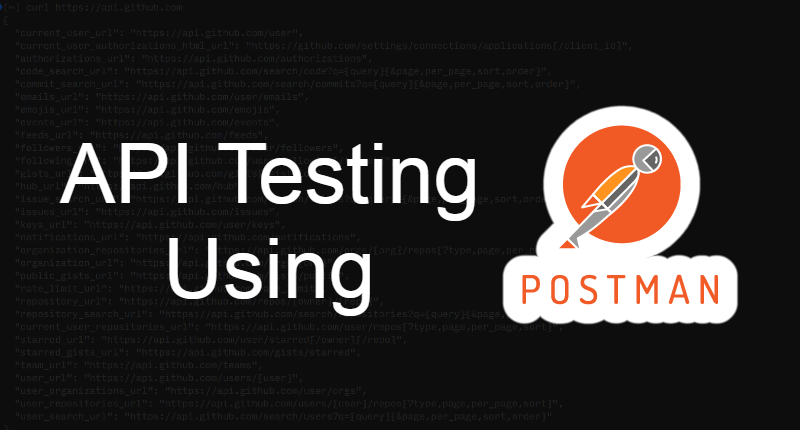
\includegraphics[width=\textwidth]{imgs/postman.png}
\end{itemize}

\noindent{\normalsize \textbf{MySQL Workbench:}}
\begin{itemize}
\item MySQL Workbench là một công cụ quản lý cơ sở dữ liệu MySQL, cung cấp giao diện đồ họa để phát triển, thiết kế và quản lý cơ sở dữ liệu một cách trực quan. Công cụ này cho phép dễ dàng tạo, chỉnh sửa cơ sở dữ liệu, thực hiện các thao tác như đảo ngược (reverse engineering) để tạo mô hình từ cơ sở dữ liệu hiện có, và chuyển tiếp (forward engineering) để triển khai mô hình thành cơ sở dữ liệu. Trong dự án Instagram clone, MySQL Workbench được sử dụng để thiết kế và quản lý cơ sở dữ liệu MySQL, bao gồm các bảng như users, posts, comments, và messages.
\end{itemize}

\noindent{\normalsize \textbf{GitHub:}}
\begin{itemize}
\item GitHub là một nền tảng quản lý mã nguồn phổ biến, cho phép các lập trình viên chia sẻ, cộng tác và quản lý phiên bản mã nguồn một cách hiệu quả. Sự phát triển của GitHub bắt đầu vào ngày 19 tháng 10 năm 2007, và trang web chính thức được ra mắt vào tháng 4 năm 2008 bởi **Tom Preston-Werner**, **Chris Wanstrath**, và **PJ Hyett**. Microsoft đã mua lại GitHub vào tháng 6 năm 2018, giúp nền tảng này có thêm nhiều nguồn lực và tích hợp sâu hơn với các sản phẩm của Microsoft, như Azure và Visual Studio. 

\item GitHub cung cấp không chỉ một kho lưu trữ mã nguồn mà còn là một công cụ mạnh mẽ để cộng tác và chia sẻ mã nguồn giữa các lập trình viên trên toàn cầu. Git, hệ thống quản lý phiên bản mà GitHub sử dụng, cho phép các lập trình viên theo dõi và kiểm soát sự thay đổi trong mã nguồn theo thời gian, giúp họ có thể quay lại các phiên bản trước nếu cần thiết và làm việc đồng thời mà không gặp phải vấn đề xung đột dữ liệu.

\item GitHub cung cấp các tính năng như **branches** (nhánh) để làm việc song song trên các tính năng hoặc sửa lỗi mà không làm ảnh hưởng đến mã nguồn chính. Người dùng có thể **fork** (tạo bản sao) các dự án từ người khác để làm việc trên đó và sau đó tạo **pull request** (yêu cầu hợp nhất) để đóng góp các thay đổi của mình vào dự án gốc.

\item GitHub cũng cung cấp các công cụ hỗ trợ như **issue tracking** (theo dõi vấn đề), **project boards** (bảng dự án), **actions** (tự động hóa quy trình phát triển), và **wikis** để tài liệu hóa các dự án, giúp các nhóm lập trình viên dễ dàng hợp tác, theo dõi tiến độ, và quản lý các vấn đề phát sinh trong suốt quá trình phát triển phần mềm.

\item Ngoài ra, GitHub còn có tính năng **GitHub Pages**, cho phép người dùng lưu trữ các trang web tĩnh trực tiếp từ kho GitHub của mình. GitHub còn hỗ trợ **private repositories** (kho lưu trữ riêng tư), giúp các lập trình viên hoặc tổ chức bảo vệ mã nguồn của họ khỏi việc chia sẻ công khai.

\item Nói chung, GitHub là một công cụ cực kỳ quan trọng trong cộng đồng lập trình viên, giúp tăng cường sự hợp tác, bảo vệ mã nguồn và thúc đẩy quy trình phát triển phần mềm nhanh chóng và hiệu quả.
\end{itemize}

\noindent{\normalsize \textbf{Giấy phép mã nguồn mở (Open Source License):}}
\begin{itemize}
    \item Giấy phép Mã nguồn mở (Open Source License) là các giấy phép cho phép người dùng tự do truy cập, sử dụng, sửa đổi và phân phối phần mềm, miễn là họ tuân theo các điều kiện của giấy phép. Các giấy phép này giúp phần mềm được phát triển và chia sẻ rộng rãi, thúc đẩy cộng đồng đóng góp vào việc phát triển phần mềm. Một số giấy phép mã nguồn mở phổ biến bao gồm: MIT License, GPL (General Public License), và Apache License 2.0. MIT License là một trong những giấy phép mã nguồn mở đơn giản nhất, cho phép người dùng sử dụng, sao chép, sửa đổi và phân phối phần mềm miễn phí, nhưng yêu cầu phải bao gồm bản quyền và thông báo giấy phép. GPL yêu cầu phần mềm phát hành dưới mã nguồn mở và bất kỳ phần mềm phát triển từ phần mềm này cũng phải tiếp tục là mã nguồn mở. Apache License 2.0 tương đối thoải mái nhưng yêu cầu bảo vệ các quyền sở hữu trí tuệ liên quan đến phần mềm. Các giấy phép mã nguồn mở thúc đẩy sự phát triển của phần mềm thông qua cộng đồng và giúp bảo vệ quyền lợi của các tác giả phần mềm.
\end{itemize}

\noindent{\normalsize \textbf{Windows Subsystem for Linux (WSL):}}
\begin{itemize}
    \item Windows Subsystem for Linux (WSL) là một tính năng trên Windows 10 và Windows Server 2019, cho phép người dùng chạy môi trường Linux trực tiếp trên Windows mà không cần phải cài đặt một máy ảo hoặc hệ điều hành dual-boot. WSL giúp các nhà phát triển sử dụng các công cụ và phần mềm Linux, ngay cả khi họ đang làm việc trên hệ điều hành Windows. WSL cung cấp một trải nghiệm người dùng rất tiện lợi vì nó cho phép sử dụng các công cụ dòng lệnh của Linux, như Bash, grep, sed, awk, và nhiều phần mềm khác mà thường chỉ có sẵn trên Linux. Điều này rất hữu ích đối với các nhà phát triển web và phần mềm, những người cần phải phát triển trên môi trường Linux mà không muốn chuyển sang hệ điều hành khác. WSL có hai phiên bản: WSL 1 và WSL 2. WSL 1 tạo ra một lớp tương thích giữa Windows và Linux, cho phép chạy các lệnh Linux trực tiếp trên Windows mà không cần máy ảo. WSL 2 cải thiện hiệu suất với một nhân Linux thực sự, giúp hỗ trợ đầy đủ các hệ thống file của Linux và tăng tốc độ đáng kể, đặc biệt là đối với các ứng dụng yêu cầu hệ thống file hoặc nhân Linux đầy đủ. 
\end{itemize}

\noindent{\normalsize \textbf{Amazon Web Services (AWS):}}
\begin{itemize}
    \item Amazon Web Services (AWS) là nền tảng dịch vụ đám mây của Amazon, cung cấp các dịch vụ như tính toán, lưu trữ, cơ sở dữ liệu, phân tích dữ liệu và các công cụ phát triển khác. AWS giúp các công ty và lập trình viên xây dựng và vận hành các ứng dụng mà không cần phải quản lý cơ sở hạ tầng vật lý. AWS cung cấp các dịch vụ đám mây quy mô lớn, đáng tin cậy, bảo mật và chi phí hiệu quả, phục vụ nhiều loại ứng dụng từ ứng dụng web đến ứng dụng di động, từ cơ sở hạ tầng IT cho đến AI và học máy. Một số dịch vụ chính của AWS bao gồm Amazon EC2 (Elastic Compute Cloud), Amazon S3 (Simple Storage Service), AWS Lambda, và Amazon RDS (Relational Database Service). Amazon EC2 cung cấp các máy ảo để bạn chạy ứng dụng, server và dịch vụ của mình. Amazon S3 là dịch vụ lưu trữ dữ liệu đám mây có khả năng mở rộng cao, giúp bạn lưu trữ và truy xuất dữ liệu một cách dễ dàng. AWS Lambda là dịch vụ tính toán không máy chủ, cho phép bạn chạy mã mà không cần phải quản lý máy chủ. Amazon RDS cung cấp các dịch vụ cơ sở dữ liệu như MySQL, PostgreSQL, và Oracle trên đám mây, giúp việc quản lý cơ sở dữ liệu trở nên dễ dàng và tiết kiệm chi phí. AWS có mô hình thanh toán theo mức sử dụng, giúp các doanh nghiệp chỉ trả tiền cho những dịch vụ mà họ sử dụng, từ đó tối ưu hóa chi phí và tài nguyên cho các công ty và tổ chức.
    
    
\includegraphics[width=\textwidth]{imgs/aws.png}
\end{itemize}

\subsubsection{ Deploy: Amazon EC2 và VPS:}
\begin{itemize}
    \item \textbf{Amazon EC2:} Amazon EC2 là dịch vụ đám mây của Amazon Web Services (AWS), cho phép người dùng thuê máy chủ ảo (instances) để triển khai và chạy ứng dụng. EC2 mang lại sự linh hoạt, khả năng mở rộng và tính sẵn sàng cao cho các ứng dụng web. Với Clone Spotify, EC2 sẽ được sử dụng để triển khai phần backend và giúp ứng dụng có thể mở rộng khi lượng người dùng tăng.
    \item \textbf{VPS:} VPS là một máy chủ ảo được phân chia từ một máy chủ vật lý duy nhất. Mỗi VPS có hệ điều hành riêng biệt, giúp triển khai ứng dụng và quản lý tài nguyên như một máy chủ độc lập. Với Clone Spotify, VPS sẽ được sử dụng cho việc triển khai các dịch vụ khác ngoài backend, như các ứng dụng phụ trợ hoặc lưu trữ dữ liệu không đụng đến hệ thống chính.
\end{itemize}